\clearpage
\section{Diagrama de Despliegue}

A continuación se describe la topología del sistema mediante un diagrama de despliegue, el cual muestra la estructura de los elementos de hardware y el software utilizado por cada uno de estos, así como las relaciones presentes entre los elementos y la forma en que se comunican entre ellos.

\begin{figure}[h]
	\centering
		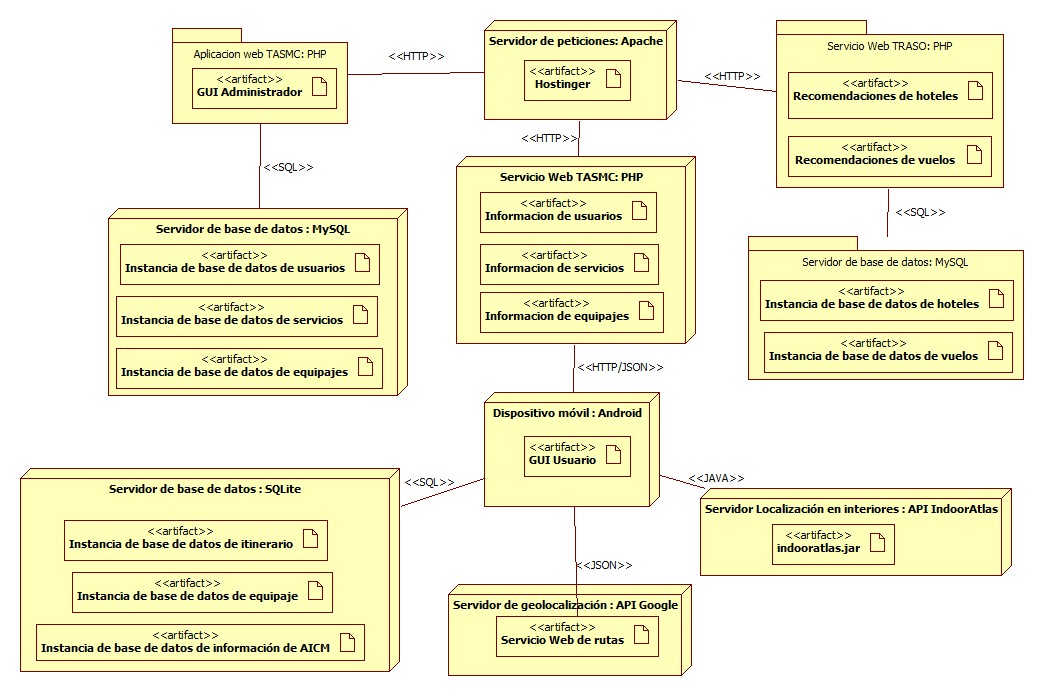
\includegraphics[width=1\textwidth]{Figuras/despliegue2.jpg}
		\rule{30em}{0.5pt}
	\caption[Diagrama de Despliegue]{Diagrama de Despliegue}
	\label{fig:diagramaDespliegue}
\end{figure}

El sistema consta de 10 elementos:

\begin{enumerate}
\item Dispositivo móvil de Android.
\item Servidor de peticiones Apache (Hostinger).
\item Servidor de base de datos MySQL de aplicación web TASMC.
\item Servidor de base de datos MySQL de servicio web TRASO.
\item Servidor de base de datos SQLite.
\item Servidor de geolocalización Google.
\item Servidor de localización en interiores IndoorAtlas.
\item Servicio web TRASO.
\item Servicio web TASMC.
\item Aplicación web TASMC
\end{enumerate}

Estos dispositivos interactúan entre sí de la siguiente manera:

El dispositivo móvil, a través de la interfaz gráfica de usuario, manda a llamar mediante consultas SQL al servidor de base de datos de SQLite para obtener instancias de equipaje, itinerario e información del AICM. Se envía una petición al servidor de geolocalización en formato JSON y llama al servicio web de rutas, además de solicitar al servicio web TRASO mediante una intercambio HTTP/JSON recomendaciones de hoteles y vuelos. Finalmente se da la interacción a través de HTTP/JSON con el servicio web propio de TASMC, que estará conectado con el servidor que se comunica con el servidor de base de datos MySQL que recibe peticiones SQL y busca instancias de usuarios, lugares y objetos que van a ser gestionados por el administrador del sistema y donde quedan registrados los lugares que serán representados en la interacción del dispositivo móvil con el servidor de localización en interiores IndoorAtlas. Los servicios web deben conectarse al servidor Hostinger al igual que la aplicación web TASMC la cual alimentará a la aplicación móvil.